\section{Jets}

\subsection{Jet clustering algorithms}

A given $pp$ collision produces many quarks and gluons.  However, because of the ``confinement principle,'' no free color charge can exist, which means no isolated quarks or gluons can exist in nature. %\cite{SM_Higgs, Particle_World}.  
It becomes energetically favorable for quark / anti-quark pairs to pop out of the vacuum to balance the color charge imbalance by forming color neutral hadrons. 
This sparks a chain reaction which produces a spray of particles in the detector. 

The anti-k$_T$ algorithm provides a way to cluster the energy deposited in the calorimeter to form a ``jet,'' and is the standard algorithm for defining jets at ATLAS \cite{antiKt}.  First it defines two quantities, 
%
\begin{equation}
d_{ij} = {\text{min}}( p_{Ti}^{-2}, p_{Tj}^{-2}) \frac{\Delta R_{ij}}{R^2} \qquad \qquad  d_i = p_{Ti}^{-2}
\end{equation}
%
where $\Delta R_{ij}^2 = (y_i - y_j)^2 + (\phi_i - \phi_j)^2$, and $R$ is the jet-radius, defined by the user.  To find the jets, the algorithm
%
\begin{itemize}
\item{Calculates $d_{ij}$ and $d_i$ for all particles in the event, and lets $d$ be the smallest $d_i$, $d_{ij}$.}
%\item{Find all the $d_{ij}$ and $d_i$ in the event, and let $d = min(\{d_{ij}, D_i\})$}
	\begin{itemize}
	\item{If $d = d_{ij}$, then it combines jet $i$ and jet $j$.}
	\item{If $d = d_{i}$, then it lets jet $i$ be the final jet.}
	\end{itemize}
\item{It continues the previous steps until all the particles in the event have been accounted for.}
\end{itemize}
%
This algorithm clusters high-$p_T$ particles together if they fall within the jet's radius. \\

The $pp$ collisions at 13~TeV typically will give rise to about 20 moderate $p_T$ jets in the detector, or around ${{20}\choose{2}} = 190$ viable di-jet candates.  So the challenge in elucidating the $H\rightarrow b\bar{b}$ or $HH \rightarrow 4b$ signals is accurately finding the ``correct'' pair(s) of jets.

Since the protons are not point-like, the colliding partons may not have equal $p_T$ in the lab frame. By definition, the net momentum will be zero in the center of mass (CM) frame.  A heavy ($\sim$TeV) resonance can be created at (or nearly at) rest in the CM frame, but when Lorentz boosting back into the lab frame the decay products can become highly collimated.  When the decay products can no longer be resolved individually, we instead search for jets with a large radius parameter (``fat jets''), indicative of merged jets \cite{SM_Higgs, Merged_Jets}.  The constituent clusters inside a fat jet are called \emph{subjets}.  
Large R (about 1.0) correspond to fat jets, and R about 0.4 correspond to the standard resolved jets.

\subsection{PFlow}

\emph{Why better?}

\textbf{To cite for pT plot:}
2007.02645 \\
Eur. Phys. J. C 81 (2021) 689

\textbf{To cite for $\phi$ plot:}
https://indico.cern.ch/event/777980/contributions/3236356/subcontributions/271401/attachments/1780062/2896765/JESJER.pdf

\begin{figure}
\centering
\subfloat[\pt resolution]{
	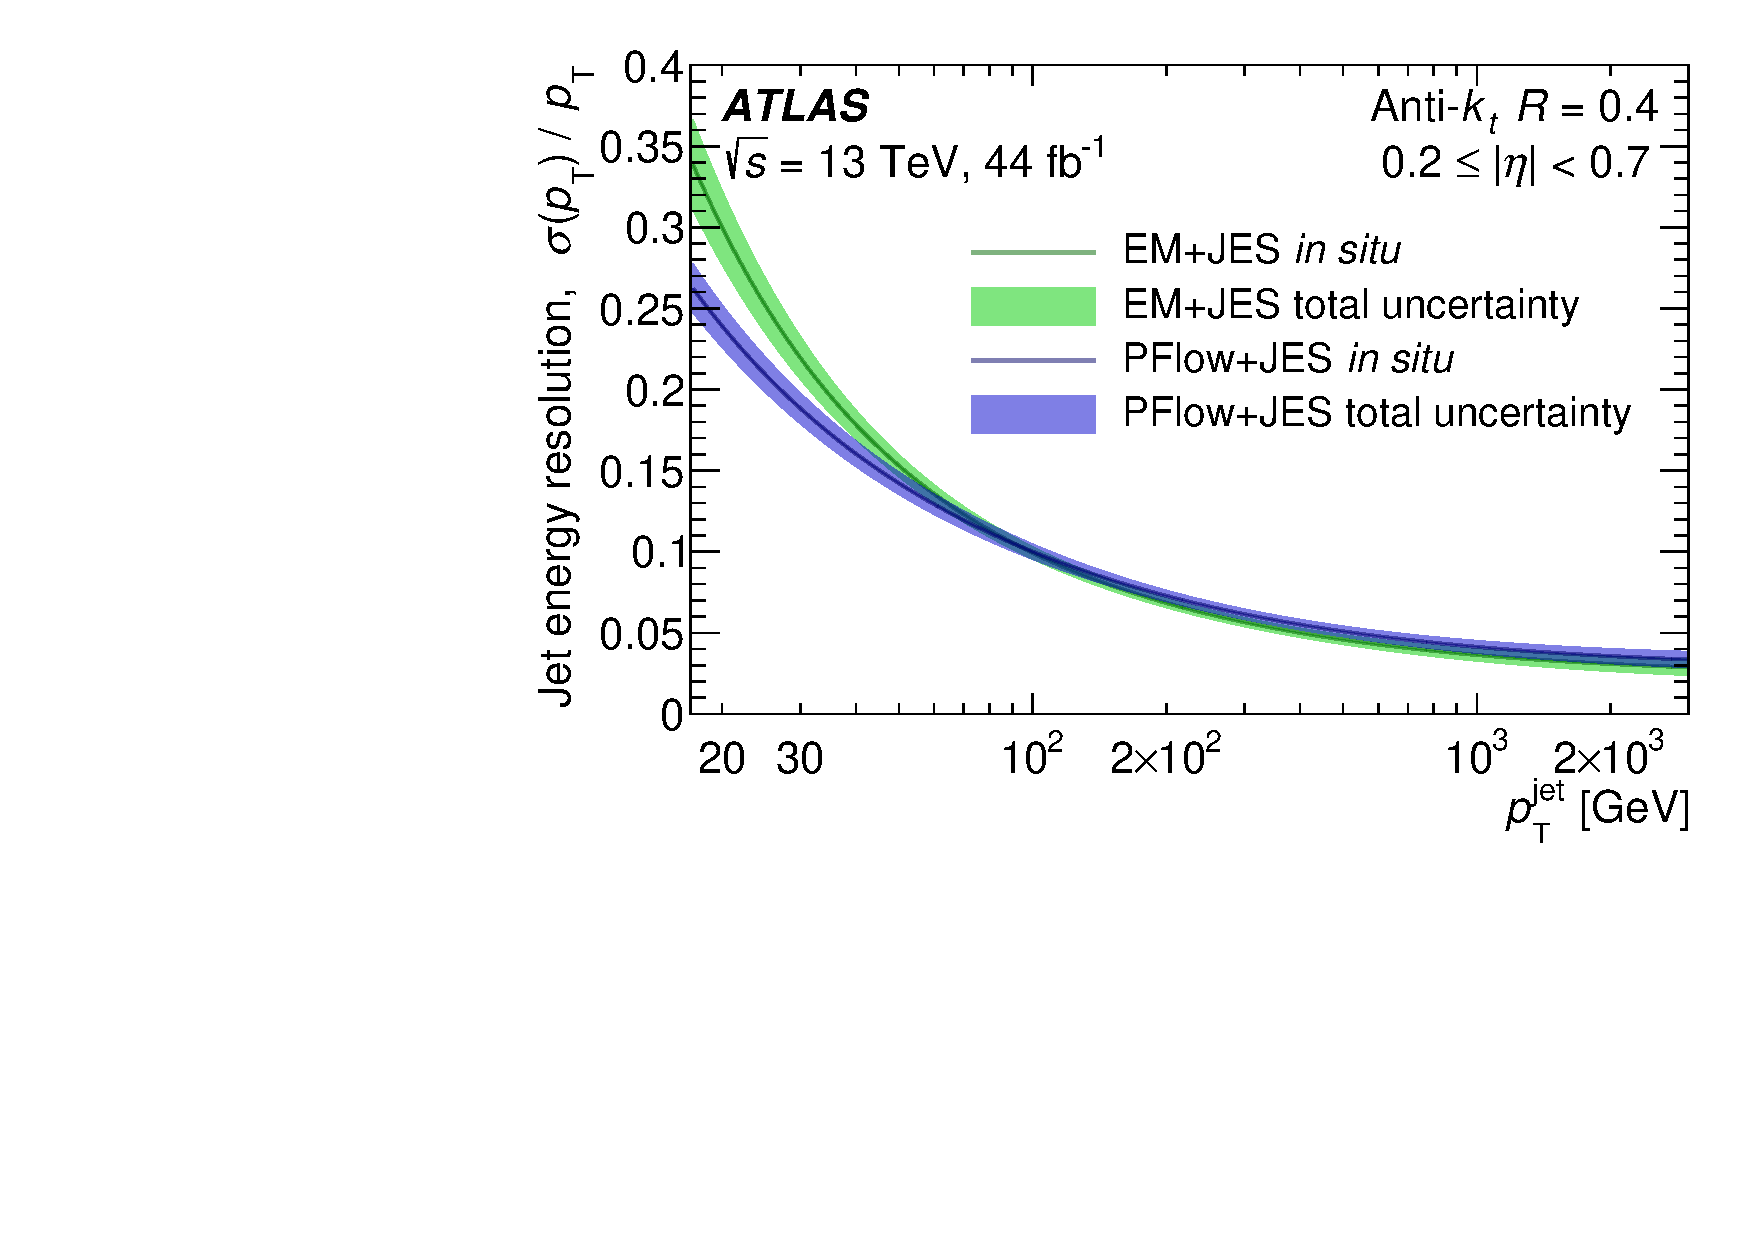
\includegraphics[height=5.4cm]{{figures/cp-graphics/jets/fig_30a}}
	\label{fig:jet-pflow-pt-res}
	}
\subfloat[$\phi$ resolution]{
	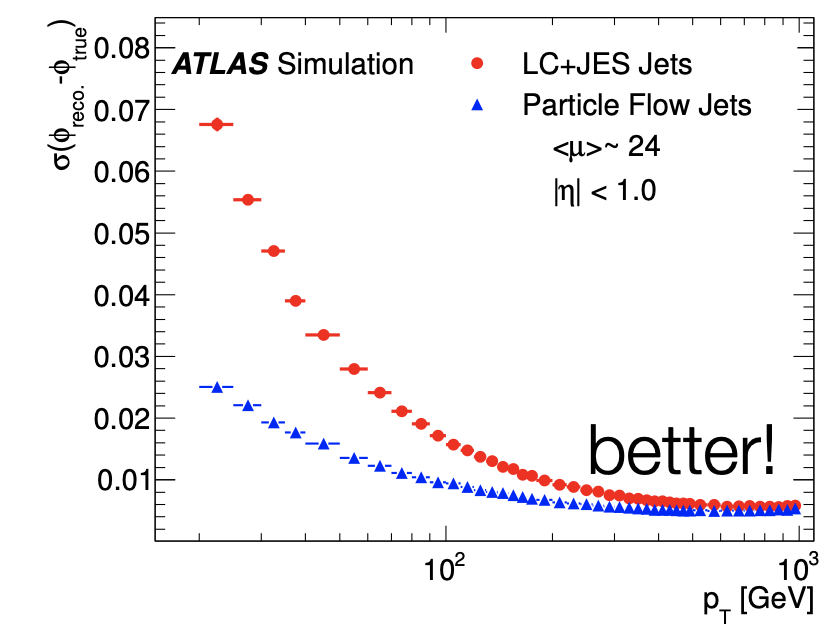
\includegraphics[height=5.4cm]{{figures/cp-graphics/jets/phi_reco}}
	\label{fig:jet-pflow-phi-res}
	}
\caption{Improvement for moving to the PFlow algorithm for jet reconstruction.}
\end{figure}

\subsection{Boosted jets}

\subsection{VR track jets}
